\documentclass{article}
\usepackage{listings}
\usepackage{graphicx}
\usepackage{float}
\usepackage[a4paper, total={6in, 9in}]{geometry}
\graphicspath{ {./} }
\usepackage{Sweave}
\begin{document}
\Sconcordance{concordance:DocGcd.tex:DocGcd.Rnw:%
1 6 1 1 0 71 1}


\title{GCD Algorithms}
\author{Bereczki Norbert Cristian}
\maketitle

\section{Algo 1: GCD by repeated subtractions}

All it is is a process of repeat subtraction, carrying the result forward each time until the result is equal to the amount being subtracted. If the answer is greater than 1, there is a GCD (besides 1). If the answer is 1, there is no common divisor (besides 1), and so both numbers are coprime, or relative prime, to each other.

The subtractive algorithm is simply this, where you 'rinse and repeat' the inner loops as long as a is not equal to b.
\begin{lstlisting}
         Do While a <> b
             Do While a > b
                 c = a - b
                 a = c
             Loop
             Do While b > a
                 c = b - a
                 b = c
             Loop
         Loop
\end{lstlisting}

\begin{figure}[H]
\caption{Performance. On Ox number of digits, on Oy time in nanoseconds}
\centering
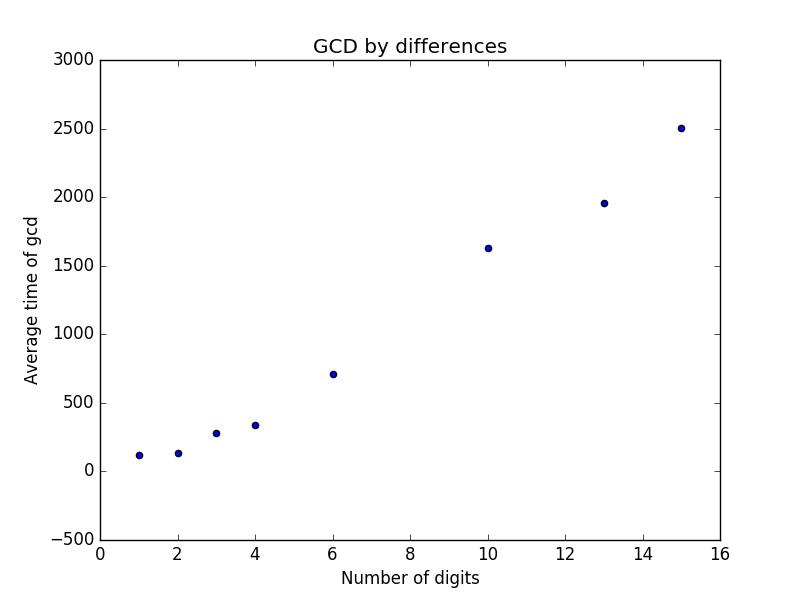
\includegraphics{GCDdifference}
\end{figure}

\newpage
\section{Algo 2: Check each number from 1 upwards if it is gcd }

You need to find the gcd of a and b.
The idea is fairly basic: you iterate from 1 to min(a,b) and check if each number can be a divisor of a and b.
If it can be then we remember the last biggest divisor, elsewhere we discard that number from being a possible answer.

The algorithm takes a lot of time because for each pair it iterates all the numbers smaller than min(a,b). So the algorithm
will take O(n) per gcd computation.

\begin{figure}[H]
\caption{Performance. On Ox number of digits, on Oy time in nanoseconds}
\centering
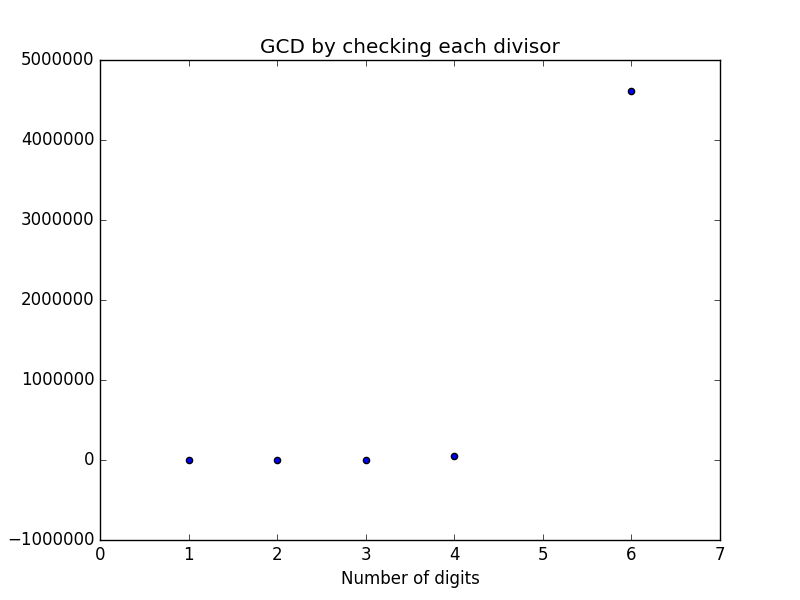
\includegraphics{GCDEach}
\end{figure}


\newpage
\section{Algo 3: Big numbers and Euclid}

The Euclidean Algorithm for finding GCD(A,B) is as follows:

\begin{enumerate}
\item If A = 0 then GCD(A,B)=B, since the GCD(0,B)=B, and we can stop.  
\item If B = 0 then GCD(A,B)=A, since the GCD(A,0)=A, and we can stop.  
\item Write A in quotient remainder form (A = B*Q + R)
\item Find GCD(B,R) using the Euclidean Algorithm since GCD(A,B) = GCD(B,R)
\end{enumerate}

Also, I applied Euclid's algorithm on big numbers.
For the big numbers I used a library, namely NTL (Number Theory Library) for C++.

\begin{figure}[H]
\caption{Performance. On Ox number of digits, on Oy time in nanoseconds}
\centering
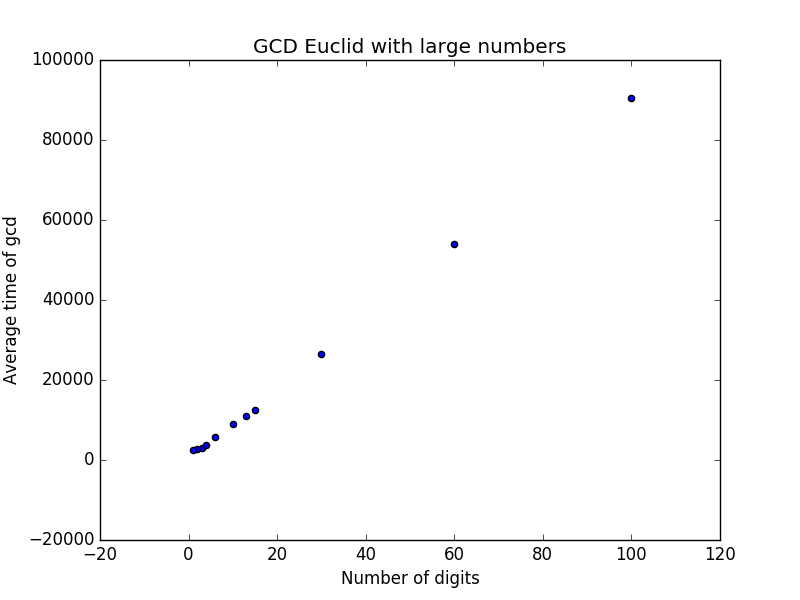
\includegraphics{GCDEuclidManyBigger}
\end{figure}



\end{document}
